\section{Theoretical Modelling of AGN Contamination}
To investigate the emission of sufficiently luminous AGN and the effect on their host galaxy, both the galaxy and AGN needed to be theoretically modelled so that a composite AGN-Galaxy could be constructed. To achieve this, we thoroughly investigated various galaxy template sets, seeking a comprehensive and reliable collection of galaxy SEDs before settling on the SWIRE \citep{polletta_spectral_2007} and GALSEDATLAS templates \citep{brown_atlas_2014}. For the AGN models, the SKIRTOR \citep{stalevski_3d_2012} set of AGN models was chosen. The selection of the most suitable models and templates for this project involved careful consideration of various factors. For the galaxy templates, it was crucial to have a comprehensive set representing the diverse types of galaxies found in the universe. Additionally, these templates needed adequate resolution so that the emission and absorption features of the galaxies were identifiable. Finally, the templates were required to possess an appropriate spectral range, spanning the entirety of the far-ultraviolet to the far-infrared regions. Comprehensive coverage and the availability of well-established, validated spectra were considered essential criteria in selecting a suitable template set. To select an appropriate set of AGN models, the most important criteria that had to be met were that the model set could be flexible enough to reproduce Type 1 and Type 2 AGN and that the wavelength coverage was similar to the galaxy templates. When selecting the set of AGN models, it was essential that the set could recreate the emission characteristics of observed AGN with the highest possible fidelity.
\subsection{Galaxy Templates}
The SWIRE template set was selected primarily for its comprehensive representation of diverse galaxy types, including elliptical galaxies across various evolutionary stages, spiral galaxies exhibiting a range of morphological features, and actively star-forming starburst galaxies. Including star-forming and starburst galaxy templates with high-resolution emission and absorption lines within the 5-12 micron spectral region further motivated the selection of the SWIRE template set. The detailed features within these templates provide valuable diagnostic capabilities for investigating the effect of AGN contamination on the intrinsic galaxy light originating from physical processes. Although the set also contained AGN templates, they were not utilised in subsequent analyses. \citep{polletta_spectral_2007}. As the SWIRE templates wavelength range is 1005 -- $6 \times 10^7$~\AA, these templates were not suitable for the use of Lyman break colour-space, which relies on the exploitation of the rest frame Lyman break, which is at 912{\AA}. During preliminary SED modelling, the SWIRE templates were only used in the UVJ colour space. The second set of templates used was the GALSEDATLAS template library. While SWIRE contained 25 semi-empirical derived templates, GALSEDATLAS covers a far more extensive wavelength range ($10^2 -$$10^7${\AA}) of 129 nearby galaxies. These templates were chosen to replace the SWIRE templates due to their broader wavelength coverage, diverse galaxy types and larger sample size \citep{brown_atlas_2014}. To simplify any calculations, the rest-frame version of these templates was used throughout the rest of this project so that redshift didn't need to be considered in the modelling. The Galaxy templates were then output with a column for wavelength ({\AA}) and total flux ($ergs\slash s\slash cm^{2}\slash ${\AA}). 
\subsection{AGN Models and Parameter Selection}
  The Fritz AGN models were initially explored due to their wide use in the literature and reasonable reproduction of AGN spectra but were abandoned in favour of the SKIRTOR models. The SKIRTOR models were chosen for their reasonably sized parameter space and use of the clumpy dust model in the solution to the radiative transfer equation to generate a spectral energy distribution. The clumpy dust model is preferred because it accurately represents observed AGN spectra more accurately than the smooth, continuous dust distribution model employed by the Fritz models \citep{gonzalez-martin_role_2023}. Each SKIRTOR model utilises the SKIRT code \citep{camps_skirt_2015} to solve the radiative transfer equation and generate an emission spectrum, incorporating a clumpy two-phase dust distribution for the dusty torus (as detailed in Section 3). We employed the SKIRTOR model set, consisting of 19,200 models covering all parameter combinations (See Table \ref{tab:skirtor_parameters}), to model the AGN.  
\begin{table}[h!]
  \centering
  \begin{tabular}{llp{5.5cm}} % Adjust the width (5.5cm) if needed
    \hline
    \textbf{Parameter} & \textbf{Symbol} & \textbf{Description and Allowed Values} \\ \hline
    Optical Depth & $\tau_{9.7\mu m}$ & Average edge-on optical depth at 9.7 $\mu$m (3, 5, 7, 9) \\
    Radial Density Exponent & $p$ & Power-law exponent for radial dust density gradient (0, 0.5, 1, 1.5) \\
    Polar Density Index & $q$ & Index for polar angle dust density gradient (0, 0.5, 1, 1.5) \\
    Opening Angle & $\theta_{open}$ & Angle between the equatorial plane and torus edge (10 to 80, steps of 10) \\
    Radius Ratio & $R_{out}/R_{in}$ & Ratio of outer to inner radius (10, 20, 30) \\
    Inclination & $i$ & Viewing angle (instrument w.r.t. AGN axis) (0 to 90, steps of 10) \\
    \hline
  \end{tabular}
  \caption{SKIRTOR AGN Model Parameters that are used in this project. While there is a large parameter space, only a certain combination of parameters produces a notable effect. Thus, the resolution of the parameter space can be reduced to find an average AGN, while the inclination can be varied to produce Type 1 or Type 2 AGN.}
  \label{tab:skirtor_parameters}
\end{table} As we are only interested in the average Type 1 and Type 2 AGN, we choose a model that best reflects this. Specifically for a Type 1 AGN, we choose an average optical depth of 7, a radial gradient of 0.5, a dust density gradient of 0, an opening angle of 40, a radius ratio of 20, and an inclination of 0. We keep the same parameters for a Type 2 AGN while varying the inclination to 90. By varying the inclination to 90, we essentially view the AGN as a Type 2 AGN as described by the Unified model of AGN. The AGN models were then output with a column for wavelength ({\AA}) and total flux ($ergs\slash s\slash cm^{2}\slash ${\AA}).
\subsection{Creating Composite SEDs}
A simplified model of the SED of a galaxy containing an AGN was considered to create composite SEDs. This model described the composite SED as a combination of the entire host galaxy SED and a portion of an AGN SED. This model was chosen as it describes the energetic output of the AGN-Host system as a combination of its constituent components. The equation below can describe the SED of such a composite galaxy
\begin{align*}
    f_{\lambda, total}(\lambda) = f_{\lambda, Galaxy}(\lambda) + \alpha \cdot f_{\lambda, AGN}(\lambda) 
\end{align*}
Here, the function $f_{\lambda}(\lambda)$ represents the SED of a particular source, and $\alpha$ is representative of the fraction of AGN SED present in the total SED of a galaxy. To construct this, both the galaxy and AGN models needed to be comparable. This was a multi-step process that involved aligning and scaling the models so that they could be used to create composite SEDs. The first step was achieved by aligning their respective SEDs to a common wavelength range, ensuring the representation of all wavelengths within both datasets. While this alignment enabled direct comparison, it necessitated the application of linear interpolation to estimate flux values at wavelengths present in one dataset but absent in the other. The interpolation process assumed a smooth, linear continuum between adjacent data points, effectively bridging gaps in the data without introducing significant artificial spectral features. The next step to ensure comparable models involved scaling the AGN to the galaxy model using integral normalisation. Integral normalisation was selected as the preferred method for establishing comparability between the template and the model. By integrating the flux over the relevant wavelength range, we calculated the total energy output for both the template and model. This approach relied on the assumption that the energy output from the AGN is comparable in magnitude to that of its host galaxy, thereby enabling the effect of the AGN model on the galaxy template to be explored by varying the AGN contribution fraction. \\\\To perform the integral normalisation process, the flux values were integrated over the wavelength range for the galaxy template and the AGN model to obtain the associated integrated flux, $F_{\lambda}$
\begin{align*}
    F_{\lambda} = \int{f_{\lambda}(\lambda)d\lambda = \int_{\lambda_{min}}^{\lambda_{max}}  f_\lambda(\lambda)d\lambda}
\end{align*}
The scaling factor was then obtained by dividing the integral of the galaxy flux by that of the AGN flux, as shown below 
\begin{align*}
    SF = \frac{F_{\lambda, Galaxy}}{F_{\lambda, AGN}}
\end{align*}
Each flux value within the AGN model was then multiplied by this scaling factor, effectively normalising and scaling its SED to align with the galaxy template (illustrated in Figure \ref{fig:combined_sed_demo}). This process allowed for a scaled AGN model suitable for constructing composite SEDs.
\begin{align*}
    f_{\lambda, total}(\lambda) = f_{\lambda, Galaxy}(\lambda) + (\alpha \cdot (f_{\lambda, AGN}(\lambda) \cdot SF) 
\end{align*}
\begin{figure}[h!]
    \centering
    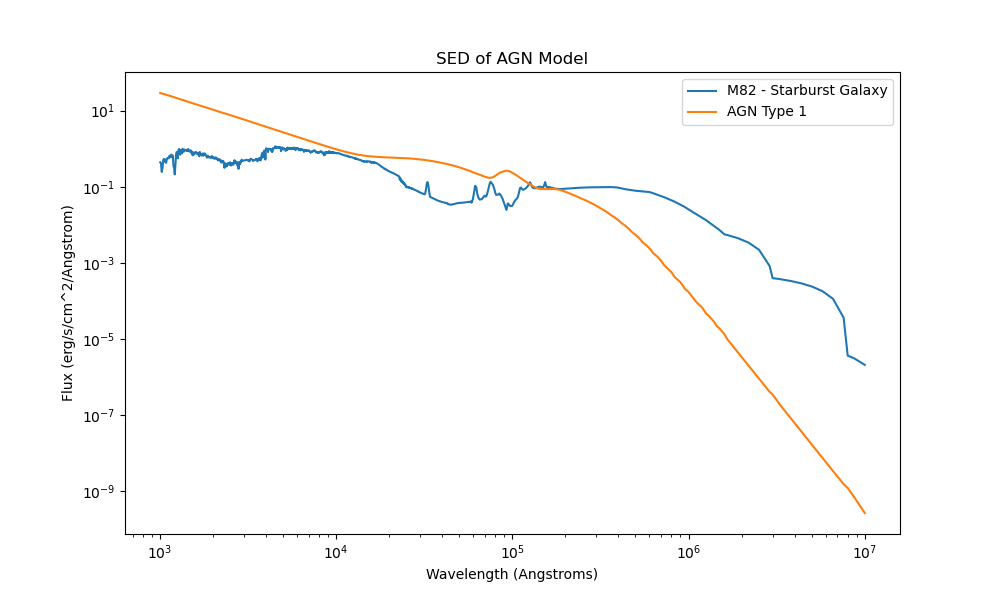
\includegraphics[width=1\linewidth]{Images/combined_sed_demo.png}
    \caption{Scaled and interpolated SEDs of a galaxy template and an AGN model, scaled using integral normalisation}
    \label{fig:combined_sed_demo}
\end{figure}
\\To construct the composite SED, a set of alpha values from 0 to 1 in steps of 0.1 was chosen, leading to 10 different composites for every galaxy-AGN combination. Given that the AGN SED has been scaled to possess a comparable total energy output to that of the galaxy, the alpha value quantifies the relative contribution of the AGN to the combined system.  For instance, an alpha value of 0.5 would correspond to an AGN contribution that is half that of the galaxy, resulting in a 2:1 ratio of galaxy-to-AGN flux. The range of alpha values was chosen as it allowed for a reasonable range of different AGN contributions to be explored; in particular, it allowed for the modelling of low-luminosity AGN in host galaxies. Finally, a comprehensive collection of composite SEDs was created, encompassing all galaxy template combinations with Type 1 and Type 2 AGN models (Figure \ref{fig:sed_agn_contaminiation}). Once all composite SEDs were generated, the subsequent step involved applying synthetic filters to these SEDs to generate synthetic photometry, which could be used to construct colour-colour diagrams for each set of filters. 
\newpage
\subsection{Synthetic Photometry and Colour-Spaces}
Synthetic photometry was required to create the colours needed for the colour-colour diagrams. We used the \texttt{astSED} functions from the \texttt{astLib} Python Library \citep{hilton_astlib_2016} with filters obtained from the SVO filter service \citep{rodrigo_svo_2020}. To ensure compatibility between the theoretical modelling and observational data from the ZFOURGE survey, we selected filters that closely matched the profiles used in ZFOURGE (See \citet{straatman_fourstar_2016} for exact filter profiles). Initially, the following synthetic bands were used to sample each SED: \texttt{U}, \texttt{V}, \texttt{J}, \texttt{u}, \texttt{g}, \texttt{r} and all four \texttt{IRAC} bands (See Table \ref{tab:filters}.)
\begin{table}[h!]
\centering
\caption{Filters used in this study with their corresponding effective wavelengths, colour spaces, and photometric systems.}
\label{tab:filters}
\begin{tabular}{lccc} 
\hline
\textbf{Filter} & \textbf{Effective Wavelength (\AA)} & \textbf{Colour-space} & \textbf{Photometric System} \\ \hline
U & 3524.66 & UVJ & Johnson \\
V & 5525.06 & UVJ & Johnson \\
J & 12393.09 & UVJ & 2MASS \\ 
3.6 & 35507.89 & IRAC & IRAC \\
4.5 & 44959.63 & IRAC & IRAC \\
5.8 & 57244.58 & IRAC & IRAC \\
8.0 & 78842.29 & IRAC & IRAC \\
u & 3569.62 & ugr & SDSS \\
g & 4711.99 & ugr & SDSS \\
r & 6285.95 & ugr & SDSS \\
\hline
\end{tabular}
\end{table}\\\\
Each synthetic filter was used to sample the SED (See Figure\ref{fig:SED_with_all_filters}) at each varying alpha level, corresponding to different levels of AGN contribution, and the appropriate colour index for each set of photometric bands was calculated. The first colour space that was constructed was the UVJ colour space.

\begin{figure}[h!]
    \centering
    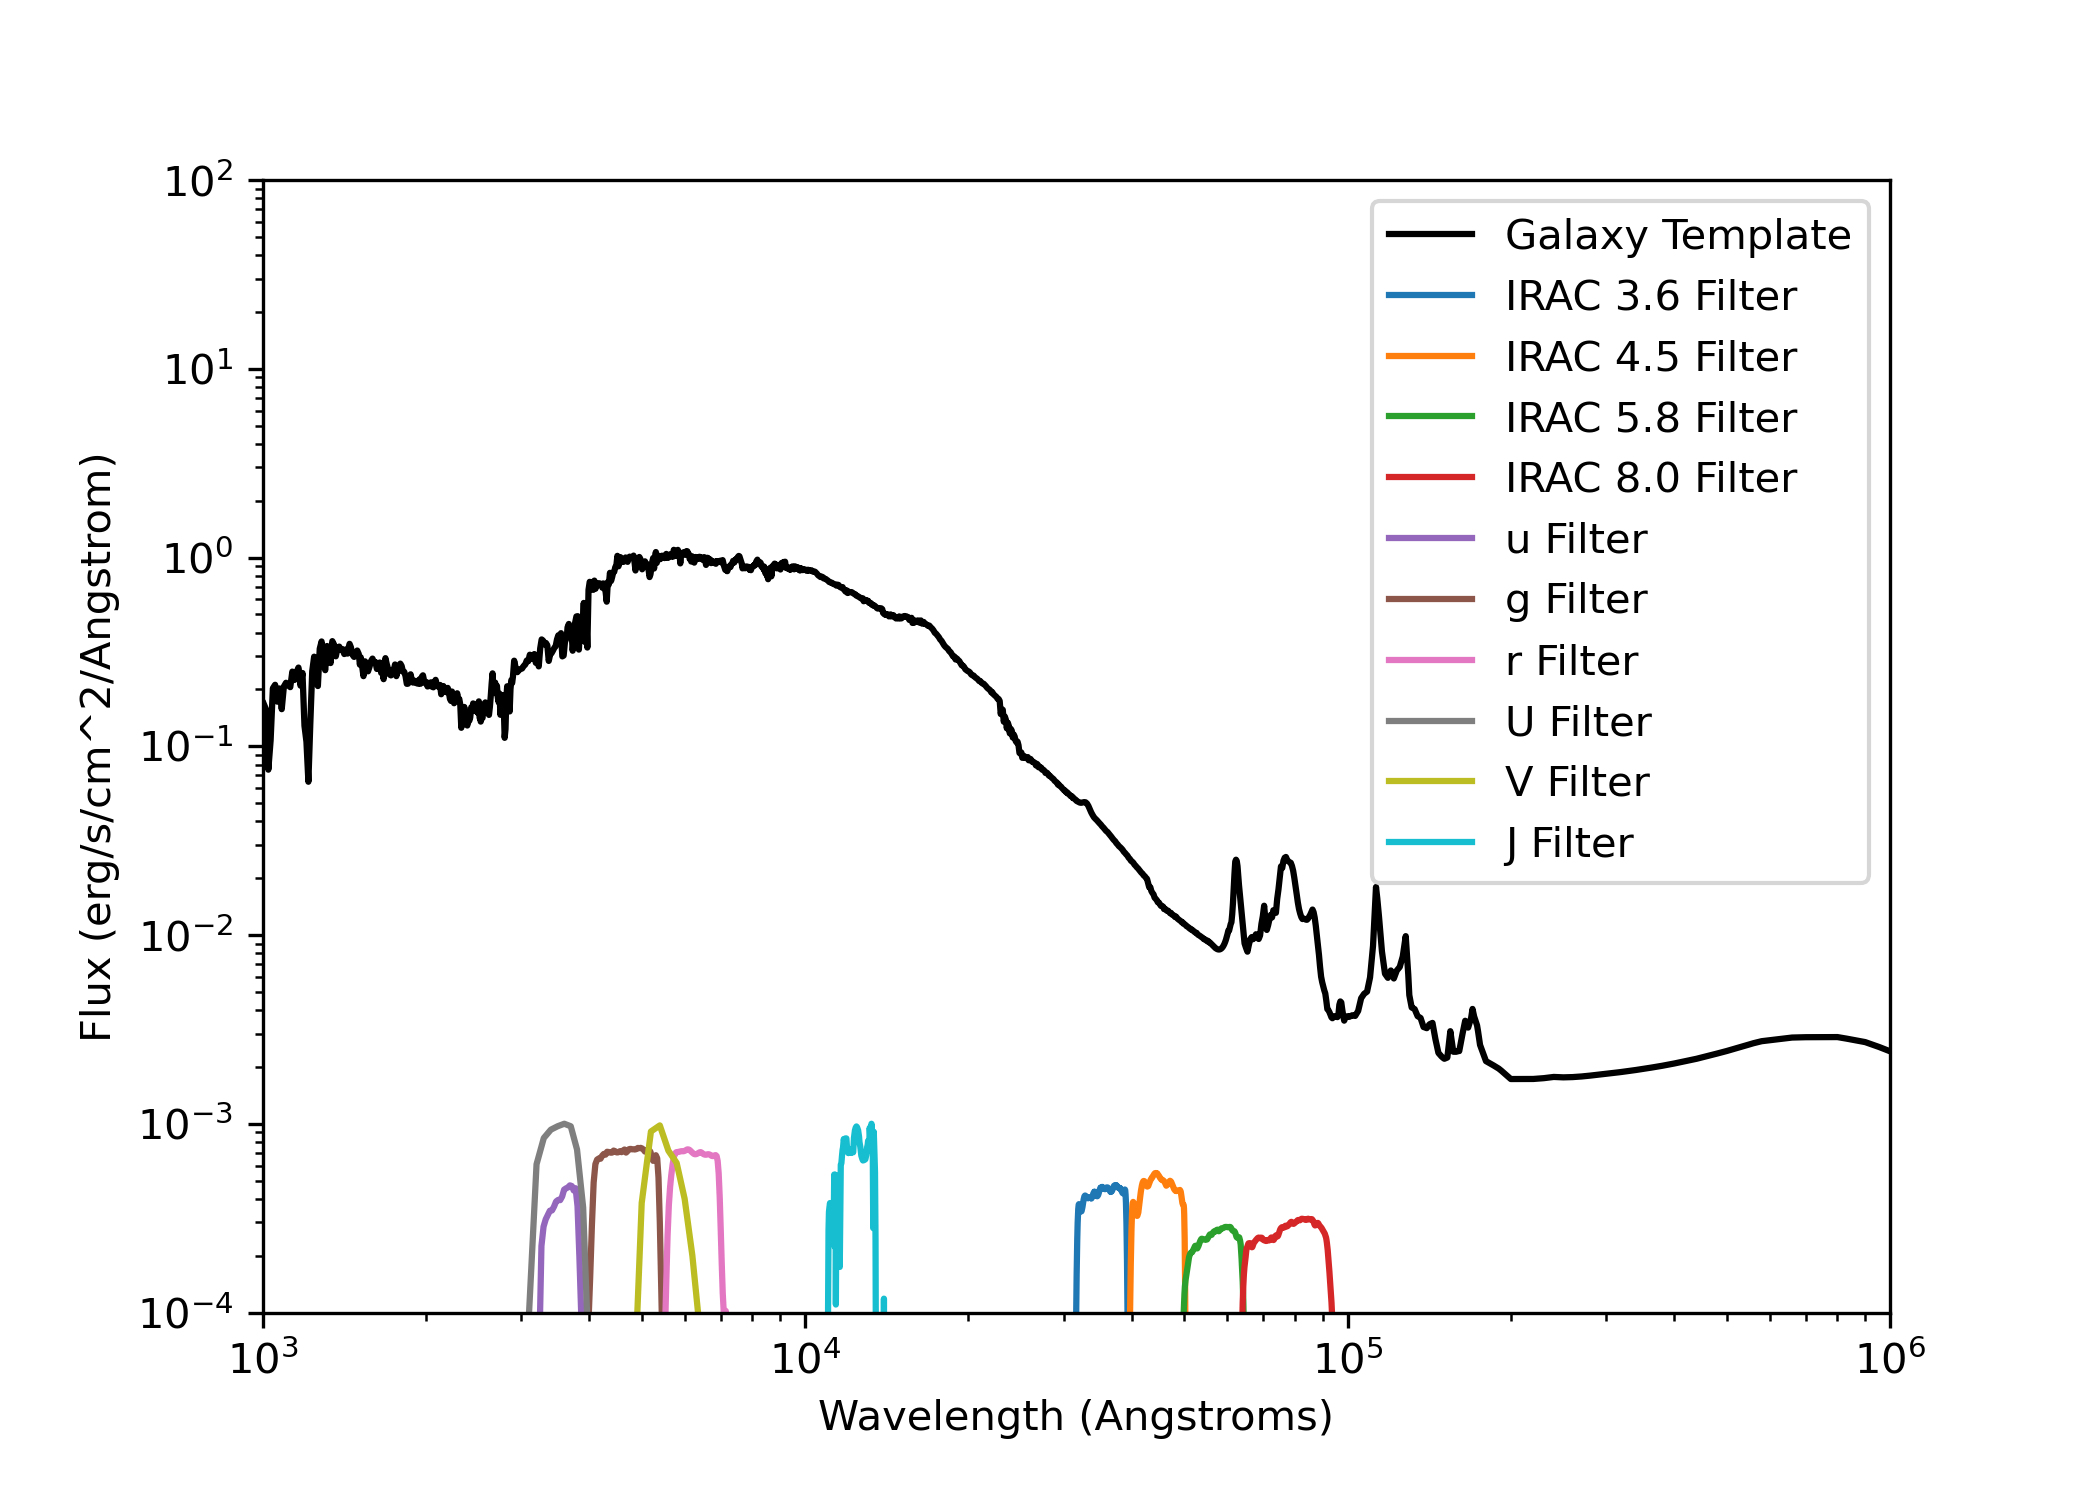
\includegraphics[width=0.8\linewidth]{Images/Galaxy SED with all filters.png}
    \caption{An example SED showing all filters used in the sampling process to create the required colours. These filters have been scaled to show where sampling takes place.}
    \label{fig:SED_with_all_filters}
\end{figure}\newpage
\subsubsection{UVJ Colour Space}
The UVJ diagram served as this work's main diagnostic tool for AGN contamination. The UVJ diagram was chosen for its simple implementation of selection regions, ability to identify dust-obscured galaxies, and use of rest-frame colours to ensure redshift-independent selection. The UVJ diagram was used to classify the composite galaxies into star-forming, quiescent, and dusty populations by categorising the composite sources based on their location in the UVJ diagram. Following the choice of the UVJ colours, the UVJ diagram was constructed by calculating the rest-frame U, V, and J colours. The colour indices were plotted with the (U-V) index on the y-axis and the (V-J) index on the x-axis, and the selection regions were included. The UVJ diagram was divided into three distinct regions. 
The quiescent region is defined by:
\begin{align*}
    (V - J, U - V) \geq (-\infty, 1.3), (0.85, 1.3), (1.6, 1.95), (1.6, +\infty)\\
\end{align*}
The remaining regions were defined by being located outside the quiescent selection region:
The star-forming region is defined by:
\begin{align*}
    (V - J, U - V) &\leq (-\infty, 1.3), (0.85, 1.3), (1.6, 1.95), (1.6, +\infty)\\
    (V - J) &\leq 1.2
\end{align*}
The dusty region is given by:
\begin{align*}
 (V - J, U - V) &\leq (-\infty, 1.3), (0.85, 1.3), (1.6, 1.95), (1.6, +\infty)\\
    (V - J) &\geq 1.2   
\end{align*}
By setting up these three selection regions, it was possible to plot each of the composite galaxies. Galaxies were classified based on their UVJ diagram position, and the proportion of each population type was then determined.
\begin{itemize}
    \item \textbf{Star-forming Fraction:}  Fraction of all galaxies in the sample classified as Star-forming galaxies.
    \item \textbf{Quiescent Fraction:} Fraction of all galaxies in the sample classified as Quiescent galaxies.
    \item \textbf{Dusty Fraction:} Fraction of all galaxies in the sample classified as dusty galaxies.
\end{itemize}
This was repeated for each set of Type 1 and Type 2 AGN-Galaxy composites at every calculated alpha value. After creating these UVJ diagrams, two other colour spaces were explored. The ugr colour space is used for redshift determination, and the IRAC colour space is used for AGN classification.
%% Need a connecting sentence that leads into the next subsection and the one after that.
\subsubsection{ugr Colour Space}
The ugr colour space was selected due to its comparable wavelength range to UVJ, which offers a broader coverage of the optical spectrum but covers a shorter wavelength range. Importantly, ugr utilizes the Lyman break caused by hydrogen absorption to determine redshift, making it particularly sensitive to UV continuum emission often associated with AGN sources. The theoretical models that were used in this project were all initially in the rest frame to test if the composite SEDs would affect the colour space. Each composite SED had to be artificially redshifted by a certain amount. To do this, astLib was used to redshift each SED composite in redshift increments of 0.1 from z = 0 to z = 4, allowing for a total of 5160 composites using the GALSEDATLAS templates as the base for the SED composites. From here, the u, g, and r colours were calculated. The colour indices were then plotted with the (U-G) index on the y and the (G-R) index on the x-axis. The Giavalisco redshift selection region was then added with the following criteria:
\begin{align*}
(U - G) &\geq 1 + (G - R); \\
(U - G) &\geq 1.6; \\
(G - R) &\leq 1.2
\end{align*}
The artificial redshift information was used to classify the composite galaxy's true redshift. This classification was then compared to the expected redshift range, as determined by the Giavilisco selection wedge. The comparison resulted in three distinct categories:
\begin{itemize}[label=\textbullet] % Use bullet points as labels
    \item \textbf{Correct Identification}: Galaxies are accurately identified inside or outside both the designated selection region and the expected redshift range.
    \item \textbf{Misidentification}: Galaxies incorrectly identified as being within the selection region; their actual redshift falls outside the expected range.
    \item \textbf{Missed Selection}: Galaxies missed by the selection process, even though their redshift is within the expected range.
\end{itemize}
The classification was performed for all composite sets and alpha values. These categories were then used to infer if an AGN affected the metrics, with larger missed selections being a potential indicator for the AGN component contaminating the ugr colour space.  The ugr colours primarily probe the ultraviolet and optical regions, suggesting that Type 2 AGN composites are not expected to exhibit significant shifts in ugr colours due to their minimal impact on ultraviolet and optical light. In contrast, Type 1 AGN, with its stronger influence on the UV and optical wavelengths, are anticipated to display noticeable colour changes. We utilised the completeness metric to evaluate the efficacy of the implemented selection methods. This metric quantifies the ability of the system to correctly identify relevant sources within a dataset. Completeness is the ratio of correctly identified sources to the total number of relevant sources, including those missed by the selection process.
\begin{align*}
\textbf{Completeness}  &= \frac{N_\text{correct}}{N_\text{correct} + N_\text{missed}}
\end{align*} 
Following the use of the ugr colour space, the IRAC colour space was then implemented to test if the composites replicated AGN colours.\\\\ 
\subsubsection{IRAC Colour Space}
The IRAC colour space was selected partly because the IRAC filters capture a significantly broader range of wavelengths than the UVJ and ugr colour spaces. Using these mid-infrared filters, the IRAC colour space was used to examine a specific portion of the electromagnetic spectrum that Type 2 AGN may influence. As the IRAC colour space is traditionally used for AGN detection, the colour space was specifically utilised to examine whether the inclusion of AGN models within galaxy templates led to an AGN identification. The colour indices were plotted, using the IRAC filters with $\log_{10} \left( \frac{f_{8.0}}{f_{4.5}} \right)$ representing the y-axis and $\log_{10} \left( \frac{f_{5.8}}{f_{3.6}} \right)$ representing the x-axis. The following criteria define the Lacy selection wedge:
\begin{align*}
    \log_{10}\left(f_{5.8}/f_{3.6}\right) &> -0.1\\
    \log_{10}\left(f_{8.0}/f_{4.5}\right) &> -0.2\\
    \log_{10}\left(f_{8.0}/f_{4.5}\right) &< 0.8 \times \log_{10}\left(f_{5.8}/f_{3.6}\right) + 0.5
\end{align*}
To plot sources on the diagram, a selection of redshifts was chosen to increase the number of AGN sources available for selection. The colour space was used to assess whether AGN was effectively selected by systematically adjusting the AGN contribution factor. It was possible to assess whether the addition of AGN to a sample increased the selection of AGN. After the selection was performed on the IRAC diagram, the completeness of the sample was calculated. Completeness is the fraction of sources identified as AGN from the entire sample composites.
\begin{align*}
    \textbf{Completeness} = \frac{N_{AGN, SEL}}{N_{AGN}}
\end{align*}
By investigating whether completeness rises with increased AGN contribution, it was possible to determine whether the theoretical composite models used in this thesis were reliably behaving as AGN candidates.
\newpage



